Nella pianificazione vengono definiti tutti i passi necessari alla conclusione del presente progetto.

\subsection{Considerazioni}\label{sec:Considerazioni}
Nel corso delle varie fasi il gruppo non mancherà di restare, ogniqualvolta necessario, in contatto con l'azienda proponente \proponente{} per poter così chiarire dubbi o accordarsi su eventuali modifiche da poter apportare ad alcuni \glo{requisiti}.\\
Si ricorda inoltre che, coerentemente con il modello scelto, si cercherà di seguire uno sviluppo di tipo incrementale. Pertanto, oltre ad una preventiva organizzazione delle parti, si procederà sempre all'implementazione per aggiunte e/o modifiche successive secondo incrementi stabiliti. Inoltre si cercherà di garantire ogni volta lo sviluppo di una versione stabile del prodotto.

\subsection{Strutturazione}\label{sec:Strutturazione}
Di seguito verrà riportata la struttura generale in cui verrà organizzato l'intero \glo{processo} di lavoro. In questo caso sono stati specificati in totale sette \glo{stadi} raggruppati essenzialmente in quattro \glo{fasi}. Per ogni stadio vengono individuati quelli che attualmente sono gli obiettivi che il gruppo \Gruppo{} si prefigge di raggiungere entro la data indicata di fine dello stesso. Nei successivi paragrafi verrà descritto ogni stadio più nel dettaglio.\\
Qui sotto viene esposto sinteticamente lo schema generale, dove ogni stadio è concettualmente collocato all'interno della rispettiva fase:

\begin{itemize}
    \item \textbf{Fase di Analisi}:
    \begin{itemize}
        \item Stadio 1 - Organizzazione preliminare;
        \item Stadio 2 - Soddisfacimento requisiti d'ingresso.
    \end{itemize}

    \item \textbf{Fase di Progettazione}:
    \begin{itemize}
        \item Stadio 3 - Strutturazione delle componenti;
        \item Stadio 4 - Concretizzazione del \glo{Proof of Concept};
    \end{itemize}

    \item \textbf{Fase di Codifica}:
    \begin{itemize}  
        \item Stadio 5 - Sviluppo e rifinitura;
        \item Stadio 6 - Qualifica e testing.
    \end{itemize}

    \item \textbf{Fase di Collaudo}:
    \begin{itemize}        
        \item Stadio 7 - Finalizzazione.
    \end{itemize}
\end{itemize}



\subsection{Stadio 1 - Organizzazione preliminare}\label{sec:Stadio1}

        \subsubsection{Periodo 1 fase di analisi}
    In questa periodo i membri del gruppo si conoscono, prendono le decisioni iniziali, valutano i capitolati, discutono sulle modalità di lavoro da adottare ed avviano la redazione dei primi documenti interni.
        \begin{itemize}
            \item \textbf{intervallo: }22 ottobre 2020 - 3 dicembre 2020;
            \item  \textbf{Figure professionali coinvolte}
                    \begin{itemize}
                        \item responsabile;
                        \item amministratore;
                        \item analista.
                    \end{itemize}
            \item \textbf{Obiettivi}
            \begin{itemize}
                \item presentazione team
                \item scelta degli strumenti ed organizzazione dell'ambiente di lavoro;
                \item scelta del nome del gruppo;
                \item approfondimento, sia individuale che collettivo, degli strumenti scelti e dei capitolati proposti;
                \item definizione e redazione delle \NdP{} e dello \glo{\SdF{}};
                \item scelta definitiva del capitolato di interesse.
            \end{itemize}
        \end{itemize}
        
        \subsubsection{Periodo 2 fase di analisi}
        Svolte le attività preliminari, il gruppo si concentra più in dettaglio sull'analisi del capitolato scelto e redige una prima stesura della documentazione esterna. 
        L'obiettivo principale di questa \glo{fase} è produrre la documentazione richiesta per il primo \glo{incontro formale} 
        di revisione programmato. La positiva conclusione di questo periodo corrisponde di fatto alla prima \glo{milestone} ufficiale del gruppo.
        
        
        \begin{itemize}
            \item \textbf{intervallo: }4 dicembre 2020 - 11 gennaio 2021;
            \item  \textbf{Figure professionali coinvolte}
                    \begin{itemize}
                        \item responsabile;
                        \item amministratore;
                        \item analista.
                    \end{itemize}
                    \item \textbf{Obiettivi}
                    \begin{itemize}
                        \item \glo{verifica} e correzione delle \NdP{} e dello \SdF{};
                        \item redazione \AdR{}:
                        \begin{itemize}
                            \item studio e definizione dei casi d'uso;
                            \item individuazione, classificazione ed analisi dei \glo{requisiti} di progetto;
                            \item definizione delle modalità di \glo{tracciamento}.
                        \end{itemize}
                        \item redazione \PdQ{};
                        \begin{itemize}
                            \item studio e definizione dei criteri qualitativi del prodotto e dei processi;
                            \item definizione dei criteri e delle modalità di verifica, di autovalutazione ed esecuzione dei test.
                        \end{itemize}
                        \item redazione \PdP{};
                        \begin{itemize}
                            \item analisi dei rischi;
                            \item scelta e definizione di un modello di sviluppo e pianificazione del lavoro;
                            \item definizione dell'organigramma generale del gruppo;
                            \item calcolo del preventivo iniziale relativo allo svolgimento del lavoro;
                        \end{itemize}
                        \item aggiornamento, verifica e correzione generale dell'intera documentazione redatta fino a questo momento;
                        \item consegna del \glo{deliverable} necessario, in vista dell'incontro con il committente per la \RR{}.
                    
                    \end{itemize}
        \end{itemize}

\subsection{Stadio 2 - Soddisfacimento requisiti d'ingresso}\label{sec:Stadio2}
Svolte le attività preliminari, il gruppo si concentra più in dettaglio sull'analisi del capitolato scelto e redige una prima stesura della documentazione esterna. L'obiettivo principale di questa \glo{fase} è produrre la documentazione richiesta per il primo \glo{incontro formale} di revisione programmato. La positiva conclusione di questo stadio corrisponde di fatto alla prima \glo{milestone} ufficiale del gruppo.
        
        \subsubsection{Periodo di svolgimento}
        4 dicembre 2020 - 11 gennaio 2021;
        
        \subsubsection{Figure professionali coinvolte}
            \begin{itemize}
                \item responsabile;
                \item amministratore;
                \item analista;
                \item verificatore.
            \end{itemize}
        
        \subsubsection{Obiettivi}
            \begin{itemize}
                \item \glo{verifica} e correzione delle \NdP{} e dello \SdF{};
                \item redazione \AdR{}:
                \begin{itemize}
                    \item studio e definizione dei casi d'uso;
                    \item individuazione, classificazione e codifica dei \glo{requisiti} di progetto;
                    \item definizione delle modalità di \glo{tracciamento}.
                \end{itemize}
                \item redazione \PdQ{};
                \begin{itemize}
                    \item studio e definizione dei criteri qualitativi del prodotto e dei processi;
                    \item definizione dei criteri e delle modalità di verifica, di autovalutazione ed esecuzione dei test.
                \end{itemize}
                \item redazione \PdP{};
                \begin{itemize}
                    \item analisi dei rischi;
                    \item scelta e definizione di un modello di sviluppo e pianificazione del lavoro;
                    \item definizione dell'organigramma generale del gruppo;
                    \item calcolo del preventivo iniziale relativo allo svolgimento del lavoro;
                \end{itemize}
                \item aggiornamento, verifica e correzione generale dell'intera documentazione redatta fino a questo momento;
                \item consegna del \glo{deliverable} necessario, in vista dell'\glo{incontro formale} con il committente per la \RR{}.
            \end{itemize}

\newpage
\subsection{Diagramma di Gantt delle attività della fase di Analisi}\label{sec:Stadio2}

\paperwidth=\pdfpageheight
\paperheight=\pdfpagewidth
\pdfpageheight=\paperheight
\pdfpagewidth=\paperwidth
\headwidth=\textheight

\begingroup 
\vsize=\textwidth
\hsize=\textheight

            \pagestyle{empty}
            \begin{figure}[h]
                \centering	
                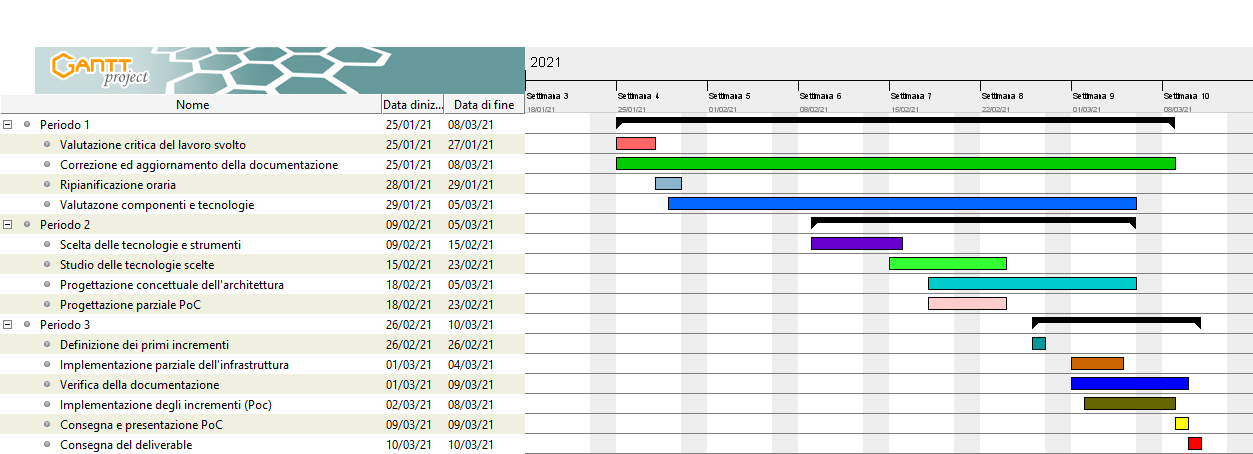
\includegraphics[height = 7cm, width = 25cm]{./src/Pianificazione/immagini/gantt_Fase1.png}
                \caption{Diagramma di Gantt delle attività della fase di Analisi}
            \end{figure}

            
\textwidth=\hsize
\textheight=\vsize

\endgroup
\newpage
\paperwidth=\pdfpageheight
\paperheight=\pdfpagewidth
\pdfpageheight=\paperheight
\pdfpagewidth=\paperwidth
\headwidth=\textwidth
    
\subsection{Stadio 3 - Strutturazione delle componenti}\label{sec:Stadio3}
       \subsubsection{Periodo 1 - Fase di progettazione}
        Una volta approvati i \glo{requisiti} di ingresso da parte del team in seguito all'aggiudicazione ufficale del capitolato, il gruppo procede verso la \glo{fase} progettuale. In questo primo periodo viene effettuata un'analisi critica del lavoro svolto. Lo scopo principale prevede la definizione degli aspetti preliminari associati allo sviluppo dell'applicazione. Inoltre si procede con la valutazione e la definizione della \glo{technology baseline}. Vengono così poste le basi per intraprendere una prima progettazione del prodotto.
        \begin{itemize}
                \item \textbf{intervallo: } 25 gennaio 2021 - 8 febbraio 2021;
                \item  \textbf{Figure professionali coinvolte}
                \begin{itemize}
                    \item responsabile;
                    \item amministratore;
                    \item progettista;
                    \item analista;
                    \item verificatore.
                \end{itemize}
                \item \textbf{Obiettivi}
                \begin{itemize}
                    \item valutazione critica di eventuali rischi riscontrati o con alta probabilità che si riscontrino;
                    \item correzione della documentazione;
                    \item ristrutturazione e correzione dell'\AdR;
                    \item valutazione delle componenti e tecnologie richieste:
                    \begin{itemize}
                        \item valutazione della fattibilità effettiva dell'utilizzo della tecnologia \glo{RFID};
                        \item contattare il proponente per alcuni chiarimenti in merito a \glo{blockchain} e \glo{NFC};
                    \end{itemize}

                    \item aggiornamento della documentazione.
                    
                \end{itemize}
        \end{itemize}


            \subsubsection{Periodo 2 - Fase di progettazione}
        
            Vengono studiate le tecnologie proposte e la loro applicabilità al fine del futuro sviluppo del prodotto, analizzandone le relative interazioni.
    
            \begin{itemize}
                \item \textbf{intervallo: }9 febbraio 2021 - 23 febbraio 2021;
            
            \item  \textbf{Figure professionali coinvolte}
                \begin{itemize}
                    \item responsabile;
                    \item amministratore;
                    \item progettista;
                    \item verificatore.
                \end{itemize}
    
                \item \textbf{Obiettivi}  
                            \begin{itemize}
                                \item scelta effettiva delle tecnologie richieste per implementare i requisiti obbligatori e critici;
                                \item studio delle tecnologie scelte coinvolte nel \glo{PoC};
                                \item definizione primi incrementi di sviluppo secondo i criteri di necessità, tipologia e quindi priorità dei requisiti.
                            \end{itemize}
                \end{itemize}          
            
                \subsubsection{Periodo 3 - Fase di progettazione}
        
                Da qui in poi si entra nella parte più specifica di costruzione del sistema. Viene quindi prodotta una prima stesura del codice con lo scopo di costruire un \glo{Proof of Concept} che utilizzi le tecnologie scelte.
        
                \begin{itemize}
                    \item \textbf{intervallo: }24 febbraio 2021 - 10 marzo 2021;
                
                \item  \textbf{Figure professionali coinvolte}
                    \begin{itemize}
                        \item responsabile;
                        \item amministratore;
                        \item progettista;
                        \item programmatore;
                        \item verificatore.
                    \end{itemize}
        
                    \item \textbf{Obiettivi}

                                \begin{itemize}
                                    \item implementazione degli incrementi definiti nel periodo 2 si veda la\hypersetup{
                                        linkcolor=blue
                                    }
                                    \hyperlink{TabellaIncrementi}{tabella degli incrementi} in appendice;
                                    \hypersetup{
                                        linkcolor=black
                                    }
                                    \item implementazione parziale componenti a supporto dell'architettura del sistema e di futuri incrementi:
                                            \begin{itemize}
                                                \item setup \glo{Kubernetes};
                                                \item \glo{backend} gestione postazioni;
                                                \item autenticazione delle \glo{API esposte};
                                            \end{itemize}
                                    \item aggiornamento, verifica e correzione generale dell'intera documentazione redatta fino a questo momento;
                                    \item consegna del \glo{deliverable} necessario, in vista dell'incontro con il committente per la \RP{}.
                                \end{itemize}
                    \end{itemize}
            

    
\subsection{Stadio 4 - Concretizzazione del \glo{proof of concept}}\label{sec:Stadio4}
Da qui in poi si entra nella parte più specifica di costruzione del sistema. Per avviare lo sviluppo questo stadio prosegue ed approfondisce la \glo{fase} di progettazione al dettaglio ed inzia quella di codifica. Viene quindi prodotta una prima stesura del codice con lo scopo di mettere insieme un iniziale prototipo stabile del sistema, avente le minime funzionalità essenziali e basilari. La sua conclusione corrisponde di fatto alla seconda \glo{milestone} principale che il gruppo \Gruppo{} intende rispettare ovvero la Revisione di Progettazione, in vista dell'incontro di revisione programmato.
        
        \subsubsection{Periodo di svolgimento}
        1 febbraio 2021 - 1 marzo 2021;
        
        \subsubsection{Figure professionali coinvolte}
            \begin{itemize}
                \item responsabile;
                \item amministratore;
                \item progettista;
                \item programmatore;
                \item verificatore.
            \end{itemize}

        \subsubsection{Obiettivi}    
        \begin{itemize}
            \item definizione completa delle strutture tramite diagrammi \glo{UML};
            \item implementazione delle componenti essenziali e obbligatorie;
            \begin{itemize}
                \item tali componenti verranno specificate più in dettaglio nei futuri aggiornamenti del presente documento, una volta stabiliti gli incrementi necessari.
            \end{itemize}
            \item progettazione di base delle \glo{interfacce} utente;
            \item \glo{verifica} del codice e delle funzionalità del prodotto;
            \item aggiornamento, verifica e correzione generale dell'intera documentazione redatta fino a questo momento;
            \item consegna del \glo{deliverable} necessario, in vista dell'incontro con il committente per la \RP{}.
        \end{itemize}
    
\subsection{Stadio 5 - Sviluppo e rifinitura }\label{sec:Stadio5}


        \subsubsection{Periodo 1 fase di sviluppo}
        Questo periodo è relativo in gran parte allo sviluppo del codice. In questa \glo{fase} principale di sviluppo ci si concentrerà non solo sugli aspetti prettamente funzionali, ma anche, e soprattuto, sui \glo{requisiti} di tipo \glo{prestazionale}. L'obiettivo principale è dunque raggiungere una versione più aggiornata, funzionante, rifinita e sufficientemente ottimizzata del prodotto.
        \begin{itemize}
                \item \textbf{intervallo obiettivo: } 17 marzo 2021 - 31 marzo 2021;
                \item  \textbf{Figure professionali coinvolte:}
                \begin{itemize}
                    \item responsabile;
                    \item amministratore;
                    \item progettista;
                    \item programmatore;
                    \item verificatore.
                \end{itemize}
                \item \textbf{Obiettivi:}
                \begin{itemize}
                    \item verifica rischi occorsi e/o potenziali nella fase ed attivare l'eventuale risoluzione o prevenenzione
                    \item definizione di tutti gli incrementi di sviluppo obbligatori da soddisfare;
                    \item correzione della documentazione secondo le direttive del committente;
                    \item implementazione incrementi appena definiti;
                    \item aggiornamento della documentazione.
                \end{itemize}
        \end{itemize}

    %    \subsubsection{Periodo 2 fase di sviluppo}
     %   A questo punto si presuppone di avere un prodotto sufficientemente funzionante ma ancora fondamentalmente incompleto. Questo periodo corrisponde ad una prima parte della \glo{fase} di \glo{validazione} ed il raggiungimento dei suoi obiettivi corrisponde alla terza \glo{milestone} principale del progetto ovvero la Revisione di Qualifica. Lo scopo di fondo è ultimare l'implementazione e concentrarsi principalmente sugli aspetti qualitativi del prodotto, in modo da consegnare infine un \glo{deliverable} conforme a quanto richiesto dal terzo incontro di revisione programmato.
      %  \begin{itemize}
       %         \item \textbf{intervallo: } 1 aprile 2021 - 15 aprile 2021;
        %        \item  \textbf{Figure professionali coinvolte}
         %       \begin{itemize}
                    %\item responsabile;
                   % \item amministratore;
                  %  \item progettista;
                 %   \item programmatore;
                %    \item verificatore.
               % \end{itemize}
              %  \item \textbf{Obiettivi}
             %   \begin{itemize}
            %        \item implementazione delle componenti restanti aggiuntive ed eventuale soddisfacimento dei \glo{requisiti} facoltativi;
           %         \item controllo, implementazione e correzione degli aspetti qualitativi del prodotto;
          %          \item mostrare un prodotto funzionante e con tutti i requisiti obbligatori soddisfatti al proponente per ricevere eventuali feedback;
         %           \begin{itemize}
        %                \item tali aspetti sono da riferirsi allo studio fatto nel documento \PdQ{}. %(potrei sbagliarmi)
       %             \end{itemize}
      %              \item copertura minima dei test all'80\% con relativo resoconto;
     %               \item \glo{verifica} del codice e delle funzionalità del prodotto;
    %                \item aggiornamento, verifica e correzione generale dell'intera documentazione redatta fino a questo momento;
   %                 \item consegna del \glo{deliverable} in vista dell'incontro con il committente per la \RQ{}.
  %              \end{itemize}
 %       \end{itemize}
        
    
\subsection{Stadio 6 - Qualifica e testing}\label{sec:Stadio6}
A questo punto si presuppone di avere un prodotto sufficientemente funzionante ma ancora fondamentalmente incompleto. Questo stadio corrisponde ad una prima parte della \glo{fase} di \glo{validazione} ed il raggiungimento dei suoi obiettivi corrispinde alla terza \glo{milestone} principale del progetto. Lo scopo di fondo è ultimare la parte di implementazione e concentrarsi principalmente sugli aspetti qualitativi del prodotto, in modo da consegnare infine un \glo{deliverable} conforme a quanto richiesto dal terzo \glo{incontro formale} di revisione programmato.
        
        \subsubsection{Periodo di svolgimento}
        8 marzo 2021 - 2 aprile 2021;
        
        \subsubsection{Figure professionali coinvolte}
            \begin{itemize}
                \item responsabile;
                \item amministratore;
                \item progettista;
                \item programmatore;
                \item verificatore.
            \end{itemize}

        \subsubsection{Obiettivi}
        \begin{itemize}
            \item correzione della documentazione secondo le indicazioni del committente;
            \item implementazione delle componenti restanti aggiuntive ed eventuale soddisfacimento dei \glo{requisiti} facoltativi;
            \item controllo, implementazione e correzione degli aspetti qualitativi del prodotto;
            \begin{itemize}
                \item tali aspetti sono da riferirsi allo studio fatto nel documento \PdQ{}. %(potrei sbagliarmi)
            \end{itemize}
            \item copertura minima dei test all'80\% con relativo resoconto;
            \item \glo{verifica} del codice e delle funzionalità del prodotto;
            \item aggiornamento, verifica e correzione generale dell'intera documentazione redatta fino a questo momento;
            \item consegna del \glo{deliverable} in vista dell'\glo{incontro formale} con il committente per la \RQ{}.
        \end{itemize}
    
\subsection{Stadio 7 - Validazione e collaudo}\label{sec:Stadio7}
L'ultimo stadio conclude la \glo{fase} di \glo{validazione} e prevede il controllo e la rifinitura generale di tutto il lavoro. L'obiettivo è perciò consegnare il progetto nella sua interezza, assicurandosi di aver soddisfatto con successo tutti i \glo{requisiti} richiesti sia dal proponente che dal committente. Gli obiettivi che si prepone fungono quindi da \glo{milestone} finale e devono essere soddisfatti conformemente a quanto richiesto dal quarto ed ultimo \glo{incontro formale} di revisione programmato.
        
        \subsubsection{Periodo di svolgimento}
        9 aprile 2021 - 3 maggio 2021;
        
        \subsubsection{Figure professionali coinvolte}
            \begin{itemize}
                \item responsabile;
                \item amministratore;
                \item progettista;
                \item programmatore;
                \item analista;
                \item verificatore.
            \end{itemize}

        \subsubsection{Obiettivi}
        \begin{itemize}
            \item correzione della documentazione secondo le direttive del committente;
            \item aggiunta e/o finalizzazione degli aspetti rimasti in sospeso o eventualmente incompleti dalle fasi precedenti;
            \item \glo{verifica} finale del codice e delle funzionalità del prodotto;
            \begin{itemize}
                \item con conseguente collaudo interno.
            \end{itemize}
            \item produzione della documentazione finale;
            \begin{itemize}
                \item aggiornamento;
                \item unificazione dei consuntivi di periodo in un consuntivo generale;
                \item redazione di un preventivo a finire dettagliato e più preciso;
                \item verifica e correzione.
            \end{itemize}
            \item consegna di tutto il \glo{deliverable}, in vista dell'\glo{incontro formale} con il committente per la \RA{}.
        \end{itemize}